\section{Future Work}


\subsection{Improve Robustness}
In this paper we have made many simplifications to the problem space just to make the placer easier to implement.
For example, our placer in its current state does not take advantage of \texttt{SLICEL}/\texttt{SLICEM} heterogeneity and simply maps all SLICE \texttt{SiteInst}s onto \texttt{SLICEL}s. 
Recall that the SLICE Sites in Xilinx FPGAs typically come in a 75-25\% split between \texttt{SLICEL}s and \texttt{SLICEM}s. 
This means that we have rendered about 25\% of the CLB fabric unusable which will inevitably hurt wirelength minimization during placement since the \texttt{SiteInst}s must be spread over a larger area. 
Enabling \texttt{SLICEL}-\texttt{SLICEM} heterogeneity can lead do greater logic density and consequently less total HPWL, but can make the packing process more complex and may contribute to higher routing congestion.

We can also add packing support for other Xilinx primitives such as the shift-register primitive \texttt{SRLx}, distributed RAM primitives \texttt{RAMSx}, or even \texttt{LATCH} primitives as discussed in \ref{sec:7_series}.
Adding support for additional primitives and macros will allow our placer to handle a wider range of HDL designs and will require deeper consideration of hardware constraints to ensure robustness.

In its current state, the prepacker and packer struggle to handle signals larger than 24-bits, especially when involved in DSP functions like addition and multiplication. 
In such designs, the Vivado synthesizer may synthesize long \texttt{CARRY4} chains with particular \texttt{EDIFHierPortInst} configurations which are currently not handled by our packer and lead to failures in the subsequent routing stage.
Further work is required to resolve these constraints in the packer.

\subsection{Force-Directed and Analytical Placement}
As discussed earlier, simulated annealing (SA) has largely been phased out in state-of-the-art (SOTA) placers due to poor scalability and long runtimes. 
Our current placer follows a straightforward \emph{prepack–pack–place} flow, with the final placement stage driven by SA. 
In future work, this stage can be retrofitted to use analytical placement (AP) while reusing the prepacker and packer. 
Here, \texttt{SiteInst}s remain the atomic placement objects, and analytical solvers can be applied to minimize the total half-perimeter wirelength (HPWL) of the connecting nets.

The following works provide a foundation for understanding AP, ranging from early formulations to modern SOTA methods:
\begin{itemize}
    \item \emph{Analytical minimization of half-perimeter wirelength} — \textbf{Kennings and Markov (2000)} \cite{AP_2000}.
    \item \emph{Kraftwerk2—A Fast Force-Directed Quadratic Placement Approach Using an Accurate Net Model} — \textbf{Spindler et al. (2008)} \cite{kraftwerk2}.
    \item \emph{Analytical placement for heterogeneous FPGAs} — \textbf{Gort et al. (2012)} \cite{AP_2012}.
    \item \emph{SimPL: An algorithm for placing VLSI circuits} — \textbf{Kim et al. (2013)} \cite{SimPL}.
    \item \emph{Multi-Electrostatic FPGA Placement Considering SLICEL–SLICEM Heterogeneity, Clock Feasibility, and Timing Optimization} — \textbf{Jing et al. (2023)} \cite{MultiElectrostatic}.
    \item \emph{OpenPARF 3.0: Robust Multi-Electrostatics Based FPGA Macro Placement Considering Cascaded Macro Groups and Fence Regions} — \textbf{Jing et al. (2024)} \cite{OpenPARF}.
\end{itemize}

As noted in Section~\ref{sec:placement}, replacing SA with AP requires splitting the placement stage into two substages:  
\emph{global placement}, which determines continuous target positions using analytical optimization, and  
\emph{detailed placement} (legalization), which snaps objects to valid \texttt{site}s while adhering to hardware constraints.  
Global placement can be performed using any number of off-the-shelf (OTS) analytical solvers.

Unlike SA, which primarily relies on heuristics and probabilistic moves, AP begins by contextualizing the problem as a collection of mathematical expressions compatible with convex optimization solvers.
As briefly introduced in Section~\ref{subsec:netlist}, a circuit netlist can be naturally modeled as a hypergraph
\begin{equation}
    G_{H} = (V_{H}, E_{H})
    \label{equ:hypergraph}
\end{equation}
where \(V_{H}\) is the set of vertices and \(E_{H}\) is the set of hyperedges, each of which may connect more than two vertices. 
In FPGA context, \(V_{H}\) corresponds to the set of \texttt{SiteInst}s placed on the \texttt{device}, while \(E_{H}\) corresponds to the set of \texttt{Net}s connecting them.

This hypergraph is reduced into a graph using one of several net models:
\begin{itemize}
    \item \textbf{Star model:} classically, introduce a virtual star node and connect it to all pins of the net. However, in electronics, we can simply use the voltage source node as the star node and avoid adding virtual nodes.
    \item \textbf{Clique model:} connect all pins of the net to each other (quadratic growth in edges). 
    \item \textbf{Bound2Bound (B2B) model:} connect only the pins at the geometric boundary (min/max in $x$ or $y$) to each other, and connect boundary pins to all interior pins. With inverse-distance weights, this model matches HPWL exactly at the point of weight calculation.
\end{itemize}

Since HPWL is direction-agnostic, directionality of FPGA nets (source/sinks) is typically ignored in reduction. Figure \ref{fig:net_model} shows an example of hyperedge reduction using the star and clique models.

\vspace{1.0cm}
{
    \centering
    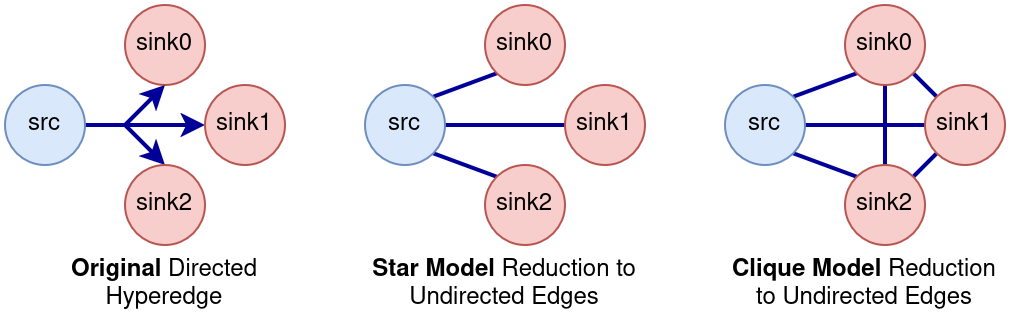
\includegraphics[width=\columnwidth]{figures/future_work/net_model.png}
    \captionof{figure}{Hyperedge reduction via Star and Clique net models.}
    \label{fig:net_model}
}
{
    \centering
    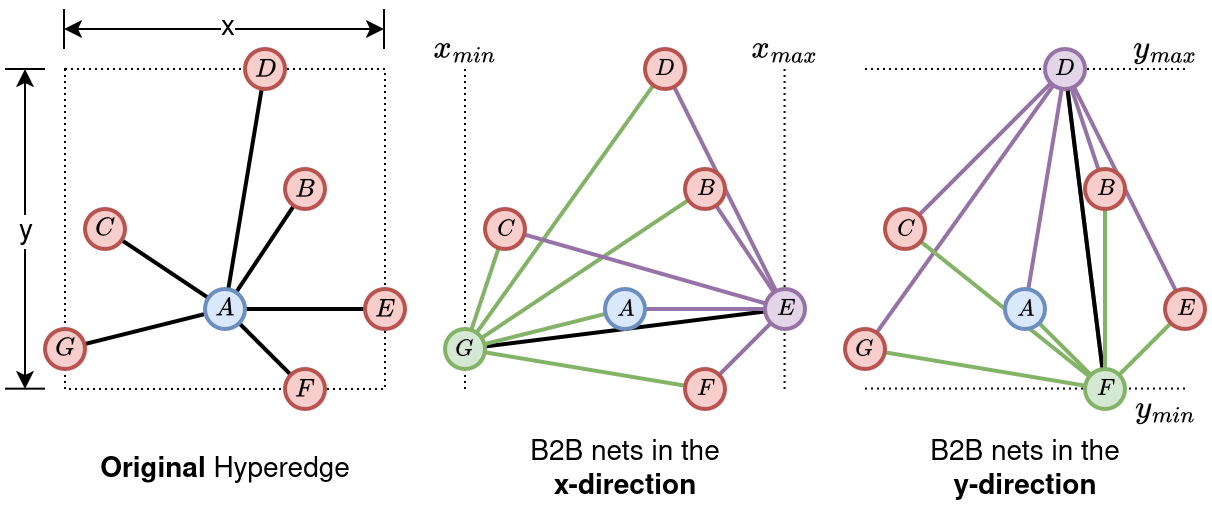
\includegraphics[width=\columnwidth]{figures/future_work/bound2bound.png}
    \captionof{figure}{Hyperedge reduction via Bound2Bound net model.}
    \label{fig:bound2bound}
}

After reduction, AP minimizes a wirelength objective, typically either a linear HPWL formulation \eqref{equ:Manhattan} or a surrogate quadratic formulation \eqref{equ:Euclidian}:

\begin{equation}
    \boldsymbol{\Phi} (\boldsymbol{x}, \boldsymbol{y}) = \sum_{i,j} w_{i,j} \left( |x_i - x_j| + |y_i - y_j| \right)
    \label{equ:Manhattan}
\end{equation}

\begin{equation}
    \boldsymbol{\Phi} (\boldsymbol{x}, \boldsymbol{y}) = \sum_{i,j} w_{i,j} \left[ (x_i - x_j)^2 + (y_i - y_j)^2 \right]
    \label{equ:Euclidian}
\end{equation}


Here, module placements in the $x$ and $y$ directions are captured by the placement vectors \( \boldsymbol{x} = (x_1, x_2, ..., x_n) \) and \( \boldsymbol{y} = (y_1, y_2, ..., y_n) \).
In both formulations, the objective function is separable with $x$ and $y$.
The weights \(w_{i,j}\) depend on both the net model and the objective:

\begin{itemize}
    \item \textbf{Star/Clique models + Quadratic objective:}  
    Assign constant weights proportional to $1$ or $1/(p-1)$ (where $p$ is the pin count) to prevent overemphasis of high-fanout nets.
    
    \item \textbf{Star/Clique models + Linear HPWL:}  
    Require iterative reweighting (e.g., $w_{i,j}=1/|x_i-x_j|$) so that the quadratic surrogate approximates the absolute value.
    
    \item \textbf{Bound2Bound + Linear HPWL:}  
    Assign weights as inverse distances, e.g.
    \begin{equation}
        w_{i,j} = \frac{1}{(p-1)\,|x_i - x_j|}
        \label{equ:weight_linearized}
    \end{equation}
    This makes the quadratic surrogate equal the HPWL for each net at the evaluation point.
\end{itemize}

The squared wirelength objective yields a unique minimizer and requires a single linear solve per iteration. 
However, it tends to over-emphasize long wires relative to short ones and tends to worsen routing demand compared to linear metrics \cite{AP_2000}. 
The linear wirelength objective more closely reflects how HPWL is measured and better correlates with routability. 
However, it is non-differentiable, so analytical placers typically handle it by iterated quadratic approximations (e.g., GORDIAN-L reweights edge coefficients each iteration) or by smooth regularizations that enable Newton-type solvers. 

For ease of implementation, it would be best to first use the squared objective before exploring the linear objective.
We can use HeAP \cite{AP_2012}, which uses the squared objective along with the B2B net model, as an instructive reference.

We can cast the squared formulation into quadratic form, which can be written compactly as
\begin{equation}
    \boldsymbol{\Phi} (\boldsymbol{x}) 
    = \tfrac{1}{2}\,\boldsymbol{x}^T \boldsymbol{Q_x}\,\boldsymbol{x} + \boldsymbol{c_x}^T \boldsymbol{x} + \text{const},
    \label{equ:quadratic}
\end{equation}
where $\boldsymbol{Q_x}$ encodes 2-pin connections between movable cells and $\boldsymbol{c_x}$ accounts for fixed terminals.  
Solving $\boldsymbol{Q_x}\boldsymbol{x} = -\boldsymbol{c_x}$ yields the optimal continuous $x$ coordinates, and the same applies independently for $y$.



\subsection{Variations on Packing}
Our current placer follows a \textbf{Site-centric} approach that resembles that of the old Xilinx ISE - the predecessor to Vivado used in the 2000s.
These days, Vivado performs \textbf{BEL-centric} placement without necessarily locking \texttt{Cell}s into \texttt{Site}s, allowing for a higher granularity of movement of \texttt{Cell}s. 
Enabling BEL-centric moveme
nt as opposed to Site-centric movement can improve HPWL minimization, but will add much more complexity to the packing and placement process to ensure robustness with respect to hardware constraints, particularly with intra-\texttt{Site} routing.

There is no constraint that forces us to pack \texttt{Cells} into \texttt{SiteInst}s before placement or to follow a strict prepacking-packing-placement flow. 
After implementing a force-directed or analytical placer, we can begin to explore different packing and placement ordering like those studied in Wuxi et al. (2019) \cite{ExplicitPacking}.

{
    \centering
    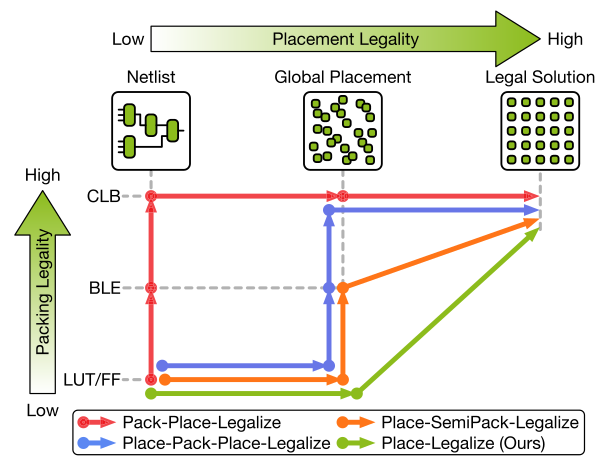
\includegraphics[width=\columnwidth]{figures/future_work/legalization.png}
    \captionof{figure}{Representative FPGA placement and packing flows. Figure taken from Wuxi et al. (2019), page 1 \cite{ExplicitPacking}}
}
\vspace{0.25cm}

\subsection{Add Hard Macro Support}
fdsa

\subsection{Parallelization}
fdsa




